\documentclass[border=10pt]{standalone}
\usepackage{tikz}
\usetikzlibrary{shapes.geometric, arrows.meta, positioning}

% Define global styles for consistent visuals
\tikzset{
    % Target Point Cloud (Static) - Blue circles
    target point/.style={circle, draw=blue, fill=blue!20, inner sep=2.5pt},
    % Source Point Cloud (Moving) - Red squares
    source point/.style={rectangle, draw=red, fill=red!20, inner sep=3pt},
    % Data Association Lines - Gray dashed lines
    match line/.style={gray, dashed, thin},
    % Final Aligned Cloud - Green squares
    aligned point/.style={rectangle, draw=green!60!black, fill=green!20, inner sep=3pt},
    % Coordinate axis style
    axis/.style={thick, ->, >=Stealth}
}

\begin{document}

% ==============================================================================
% FIGURE 1: Data Association & Initial State (Step 1)
% Description: Show Initial misalignment and nearest-neighbor matches.
% ==============================================================================
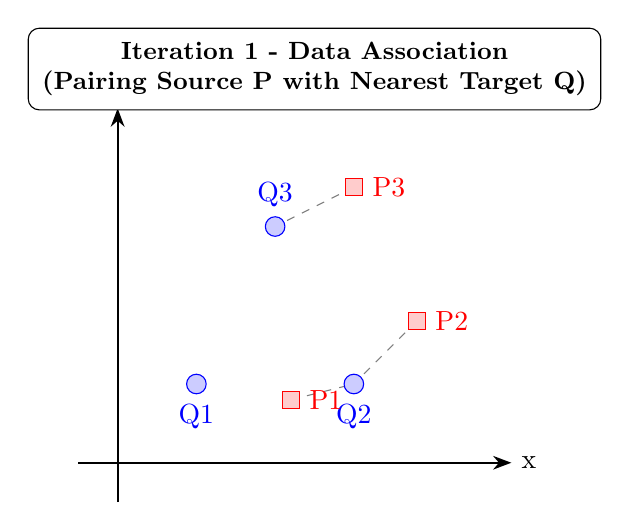
\begin{tikzpicture}
    % --- Set up coordinates ---
    % Target Cloud Q (Static Triangle)
    \coordinate (Q1) at (1,1);
    \coordinate (Q2) at (3,1);
    \coordinate (Q3) at (2,3);

    % Source Cloud P (Initial Mismatch - Rotated/Translated)
    \coordinate (P1) at (2.2, 0.8); % Closest to Q2
    \coordinate (P2) at (3.8, 1.8); % Closest to Q2 (Mismatch!)
    \coordinate (P3) at (3.0, 3.5); % Closest to Q3

    % --- Draw Data Association (Matches) ---
    % Line P1 -> closest neighbor (Q1 or Q2? Let's check: dist(P1,Q2) is smallest)
    \draw[match line] (P1) -- (Q2); 
    % Line P2 -> closest neighbor (Q2) - This is a classic mismatch example
    \draw[match line] (P2) -- (Q2);
    % Line P3 -> closest neighbor (Q3)
    \draw[match line] (P3) -- (Q3);

    % --- Draw Point Clouds ---
    % Target Q (Blue Circles)
    \node[target point, label={[blue]below:Q1}] at (Q1) {};
    \node[target point, label={[blue]below:Q2}] at (Q2) {};
    \node[target point, label={[blue]above:Q3}] at (Q3) {};

    % Source P (Red Squares)
    \node[source point, label={[red]right:P1}] at (P1) {};
    \node[source point, label={[red]right:P2}] at (P2) {};
    \node[source point, label={[red]right:P3}] at (P3) {};

    % --- Setup Canvas & Title ---
    \draw[axis] (-0.5,0) -- (5,0) node[right] {x};
    \draw[axis] (0,-0.5) -- (0,4.5) node[above] {y};
    
    % Title/Caption Area
    \node[draw, fill=white, rounded corners, inner sep=5pt, font=\small\bfseries, align=center] at (2.5, 5.0) 
        {Iteration 1 - Data Association\\ (Pairing Source P with Nearest Target Q)};

\end{tikzpicture}


% ==============================================================================
% FIGURE 2: After Iteration 1 - Apply Transformation (Step 3)
% Description: Source P' has moved closer to Q based on matches from Figure 1.
% ==============================================================================
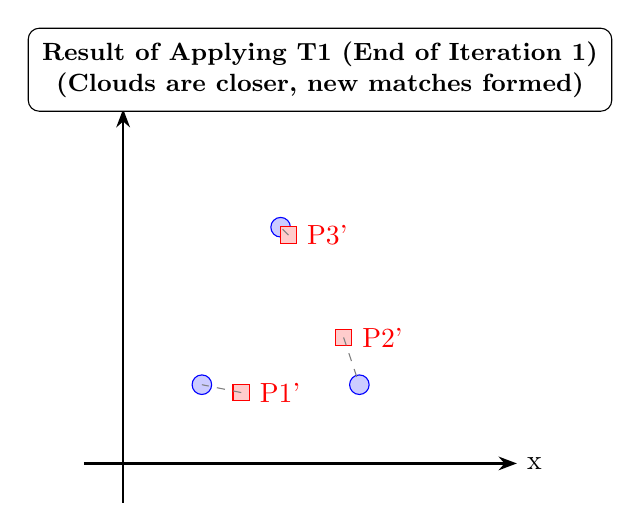
\begin{tikzpicture}
    % --- Set up coordinates ---
    % Target Cloud Q (Static Triangle - same as Fig 1)
    \coordinate (Q1) at (1,1);
    \coordinate (Q2) at (3,1);
    \coordinate (Q3) at (2,3);

    % Source Cloud P' (Transformed after Iteration 1)
    % Based on matches P1->Q2, P2->Q2, P3->Q3, the centroid of matches 
    % will pull the source cloud left and down.
    \coordinate (P1_t) at (1.5, 0.9); 
    \coordinate (P2_t) at (2.8, 1.6);
    \coordinate (P3_t) at (2.1, 2.9); % Almost matches Q3

    % --- Draw Point Clouds ---
    % Target Q (Blue Circles)
    \node[target point] at (Q1) {};
    \node[target point] at (Q2) {};
    \node[target point] at (Q3) {};

    % Transformed Source P' (Red Squares)
    \node[source point, label={[red]right:P1'}] at (P1_t) {};
    \node[source point, label={[red]right:P2'}] at (P2_t) {};
    \node[source point, label={[red]right:P3'}] at (P3_t) {};

    % --- Draw NEW Data Association ---
    % Now P2' is closest to Q2, P1' is closest to Q1
    \draw[match line] (P1_t) -- (Q1);
    \draw[match line] (P2_t) -- (Q2);
    \draw[match line] (P3_t) -- (Q3);

    % --- Setup Canvas & Title ---
    \draw[axis] (-0.5,0) -- (5,0) node[right] {x};
    \draw[axis] (0,-0.5) -- (0,4.5) node[above] {y};
    
    \node[draw, fill=white, rounded corners, inner sep=5pt, font=\small\bfseries, align=center] at (2.5, 5.0) 
        {Result of Applying T1 (End of Iteration 1)\\ (Clouds are closer, new matches formed)};

\end{tikzpicture}


% ==============================================================================
% FIGURE 3: Convergence (Step 4 / Final Result)
% Description: The clouds match, error is low, loop stops.
% ==============================================================================
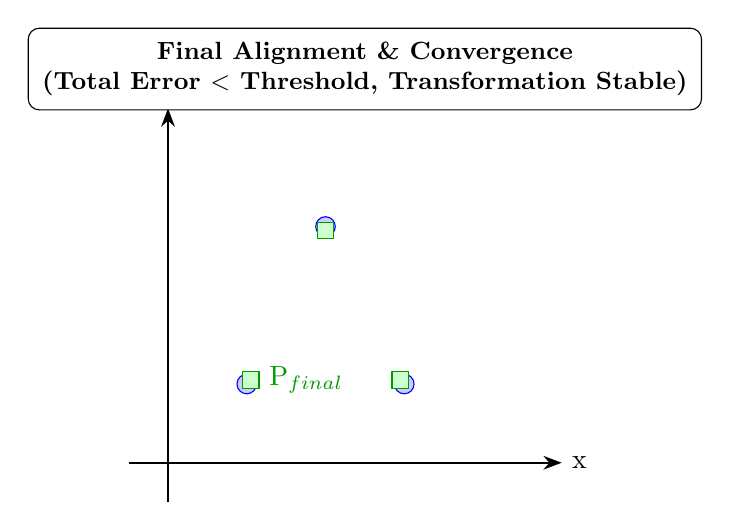
\begin{tikzpicture}
    % --- Set up coordinates ---
    % Target Cloud Q (Static Triangle)
    \coordinate (Q1) at (1,1);
    \coordinate (Q2) at (3,1);
    \coordinate (Q3) at (2,3);

    % Final Converged Source Cloud P_final
    % (Slight error added to show they are separate but aligned)
    \coordinate (Pf1) at (1.05, 1.05); 
    \coordinate (Pf2) at (2.95, 1.05);
    \coordinate (Pf3) at (2.00, 2.95);

    % --- Draw Point Clouds ---
    % Target Q (Blue Circles)
    \node[target point] at (Q1) {};
    \node[target point] at (Q2) {};
    \node[target point] at (Q3) {};

    % Final Source P_final (Green Squares)
    \node[aligned point, label={[green!60!black]right:P$_{final}$}] at (Pf1) {};
    \node[aligned point] at (Pf2) {};
    \node[aligned point] at (Pf3) {};

    % --- Setup Canvas & Title ---
    \draw[axis] (-0.5,0) -- (5,0) node[right] {x};
    \draw[axis] (0,-0.5) -- (0,4.5) node[above] {y};
    
    \node[draw, fill=white, rounded corners, inner sep=5pt, font=\small\bfseries, align=center] at (2.5, 5.0) 
        {Final Alignment \& Convergence\\ (Total Error $<$ Threshold, Transformation Stable)};

\end{tikzpicture}

\end{document}